% Created 2021-01-04 Mon 14:51
% Intended LaTeX compiler: pdflatex
\documentclass[11pt]{article}
\usepackage[utf8]{inputenc}
\usepackage[T1]{fontenc}
\usepackage{graphicx}
\usepackage{grffile}
\usepackage{longtable}
\usepackage{wrapfig}
\usepackage{rotating}
\usepackage[normalem]{ulem}
\usepackage{amsmath}
\usepackage{textcomp}
\usepackage{amssymb}
\usepackage{capt-of}
\usepackage{hyperref}
\author{Serge Stinckwich}
\date{\today}
\title{Kendrick Meta-model v3}
\hypersetup{
 pdfauthor={Serge Stinckwich},
 pdftitle={Kendrick Meta-model v3},
 pdfkeywords={},
 pdfsubject={},
 pdfcreator={Emacs 28.0.50 (Org mode 9.4.4)}, 
 pdflang={English}}
\begin{document}

\maketitle

\section{Kendrick Meta-Model Diagram}
\label{sec:orgfc5378f}
\begin{center}
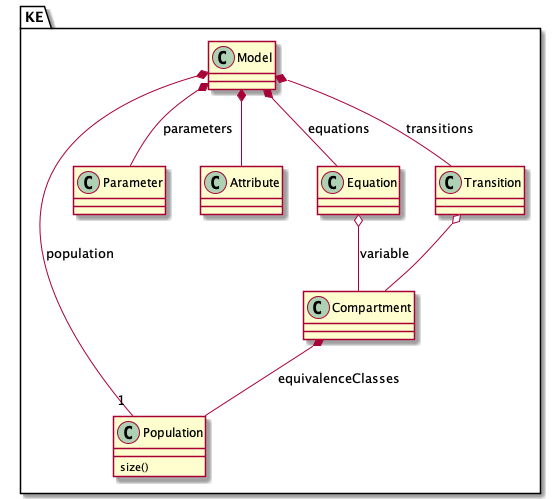
\includegraphics[width=.9\linewidth]{meta-modelv3.png}
\end{center}

\section{Kendrick Meta-model description}
\label{sec:orgd880a98}

The abstract syntax of Kendrick is based on the mathematical definitions of Kendrick
and relies on an object-oriented meta-model.
We use the UML graphical modelling language to describe the Kendrick meta-model.

\subsection{Model}
\label{sec:org31f7abb}
A Kendrick \textbf{model} (instance of KEModel) is defined by a collection of \textbf{transitions}, a collection of \textbf{parameters}, a collection of \textbf{attributes}, a collection of \textbf{equations} and one \textbf{population}.

In the implementation, equivalence relations are restricted to equalities on individuals' attributes.
This guarantees that each equivalence class (the individuals with the same values for a given set of attributes) has a known name: the ordered set of attribute names used in the equality.
An attribute is simply a partial function on the population to any domain with equality. The function is assumed total on the compartments it defines.
When models are combined, attribute names must stay unique in the whole population (name clashes must be avoided).

\subsection{Concern}
\label{sec:org45f2a76}
Do we need to introduce \textbf{concern} concept in the meta-model ?

\subsection{Population}
\label{sec:org24a2b2c}
A Kendrick \textbf{population} (instance of KEPopulation) is defined by a collection of \textbf{compartments} i.e. of equivalence classes.
A population has a method size (number of individuals of that population).
The size of the population is the sum of the sizes of each compartment.
A new population is empty (size = 0).

\subsubsection{Issues to be solved:}
\label{sec:org38a2a9f}
\begin{itemize}
\item Why compartments are represented as a set of dictionaries with a specific structure (linked to the fact that there is no compartment class).
\item Why we can add/remove individuals or have access to the individuals from population ?
\item What is diedInList ?
\end{itemize}

\subsection{Compartment}
\label{sec:org637f939}
At the moment, we have no class \textbf{compartment}, this is bit weird because compartment are represented as Dictionary.

\subsubsection{Issues to be solved:}
\label{sec:orgb214871}
\begin{itemize}
\item Represent compartment as object and not Dictionary (issue 89).
\end{itemize}

\subsection{Attribute}
\label{sec:orgdf207ca}
An attribute is not defined by a class. Examples of attributes are: \#species, \#status.
A Kendrick \textbf{attribute} has a name and a domain.

\subsection{Functional rates}
\label{sec:org4dd5f83}
Apparently there is no representation of functional rates in the K meta-model.
Do we need to introduce it ?

The following concepts are not fondamental to Kendrick, but allow to represents ODEs.
\subsection{Equation}
\label{sec:org392f406}
A Kendrick \textbf{equation} (instance of KEEquation) represent an ODE (Ordinary Differential Equation). It is defined by a \textbf{variable} that depends on time 

\subsubsection{Issues to be solved:}
\label{sec:org19a4a5c}
\begin{itemize}
\item Do we need equation and transition, because normally they can be generated from each others ?
\end{itemize}

\subsection{Variable}
\label{sec:org5759923}
   A Kendrick \textbf{variable} (instance of KEVariable) represent a mathematical variable in an equation.
A variable is defined with a name (symbol).

\subsubsection{Issues to be solved:}
\label{sec:org3fd02f3}
\begin{itemize}
\item variable name is called symbol in the implementation that is not really informative.
\item there is no dependency between variables. In order to know the dependency we have to look at the \textbf{equation} that contains the variable.
A variable should have a list of dependencies.
\end{itemize}

\url{Kendrick\_Meta-model\_description/2020-07-16\_17-49-49\_ReHab\_Pharo.st}

\subsection{Parameter}
\label{sec:orgafdd3bf}
   A Kendrick \textbf{parameter} (instance of KEParameter) represent parameters in an epidemiological model.
A parameter is defined with a name (symbol) and an expression.
By default, a Kendrick model got a \textbf{\textbf{N}} parameter initialized with the cardinality of the whole population of a model.

\subsubsection{Issues to be solved:}
\label{sec:orgdca904d}
\begin{itemize}
\item \url{https://github.com/UMMISCO/kendrick/issues/99}
\item This is not really clear why we separated variables and parameters. Apparently parameter are not depending on another variable.
\end{itemize}

\section{Kendrick Workflow Meta-model description}
\label{sec:org3fe21c1}
\section{Smalltalk implementation}
\label{sec:orgced1d9c}
Functional rates are represented as lexical closure in Smalltalk.

\subsection{Attribute}
\label{sec:org2f65e19}
   Attributes are Smalltalk symbol (immutable String).
   Domain associated to attributes are defined as Smalltalk symbol also.
You add all the attributes with attributes: method
\begin{verbatim}
model := KEModel new.
model attributes: {(#status -> #(#S #I #R). (#species -> #(#human #bird))}.
\end{verbatim}

or add attributes one by one with: addAttribute:value:
\begin{verbatim}
model := KEModel new.
model addAttribute: #status value: #(#S #I #R).
model addAttribute: #species value: #(#human #bird).
\end{verbatim}
\end{document}